\section{Histogramme und deren Anwendungen}

    \subsection{Histogramme}
        Sei $u:\Omega \to F$ ein diskretes Bild, dann heißt die Abbildung
        \[H_u : F \to \N_0\]
        \[F \ni k \mapsto \# \{x \in \Omega \mid u(x) = k\}\]
        \textbf{Histogramm}\index{Histogramm} des Bildes $u$. Dieses gibt an, wie oft der Helligkeitswert $k$ im Bild $u$ vorhanden ist.\\
        Damit gilt auch:
        \[\sum_{k \in F}H_u(k)=\abs{\Omega} \text{, also die Anzahl der Pixel}.\]
        \begin{bemerkung*}
            Manchmal betrachtet man die relative Häufigkeit $\widetilde H_u(k) =\displaystyle  \frac{H_u(k)}{\abs{\Omega}}$.
        \end{bemerkung*}

        \pa{\large Beispiel:}

        \begin{center}
            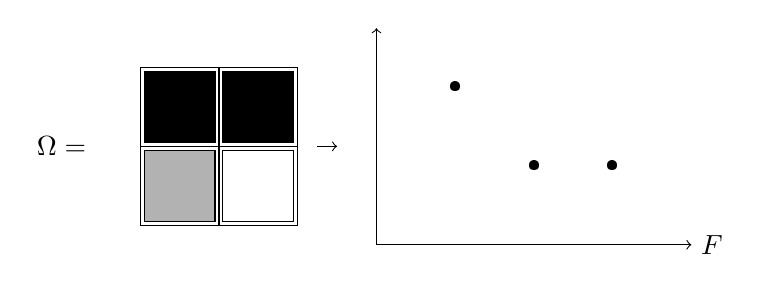
\begin{tikzpicture}
                \draw (0,0) node {$\Omega=$};
                \draw[fill = black] (1.05,0.95) rectangle (1.95,0.05);
                \draw[fill = black] (2.05,0.95) rectangle (2.95,0.05);
                \draw[fill = black!30] (1.05,-0.05) rectangle (1.95,-0.95);
                \draw[fill = white] (2.05,-0.05) rectangle (2.95,-0.95);
                \draw (1,1) grid (3,-1);
                \draw[->] (3.25,0) -- (3.5,0);
                \draw[->] (4,-1.25) -- (8,-1.25) node[right] {$F$};
                \draw[->] (4,-1.25) -- (4,1.5);
                \tvmark{5}{-1.25}{black}
                \tvmark{6}{-1.25}{\vphantom{b}grey}
                \tvmark{7}{-1.25}{white}
                \thmark{4}{-0.25}{1}
                \thmark{4}{0.75}{2}
                \draw (5,0.75) node {\textbullet};
                \draw (6,-0.25) node {\textbullet};
                \draw (7,-0.25) node {\textbullet};
            \end{tikzpicture}
        \end{center}

        Für kontinuierliche Bilder wird  das allgemeinere Konzept des \textbf{Maßes}\index{Maß} benötigt:
        \begin{center}
            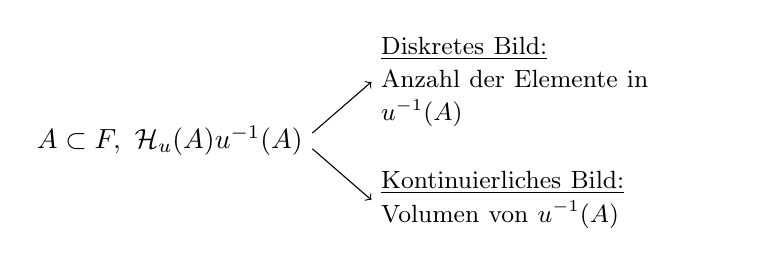
\begin{tikzpicture}
                \draw (0,0) node[left] {$A \subset F, \ \mathcal H_u(A)  \coloneqq  \abs{u^{-1}(A)}$};
                \draw[->,text width = 4.5cm] (0,0.1) -- (0.75,0.75) node[right] {\small \underline{Diskretes Bild:}\\ Anzahl der Elemente in $u^{-1}(A)$};
                \draw[->,text width = 4.5cm] (0,-0.1) -- (0.75,-0.75) node[right] {\small \underline{Kontinuierliches Bild:}\\ Volumen von  $u^{-1}(A)$};
            \end{tikzpicture}
        \end{center}

        Zusammenhang zum vorherigen: $\displaystyle \mathcal H_u(A) = \sum_{k \in A} H_u(k)$.
        Man sagt dann, dass $H_u$ eine \textbf{Dichte}\index{Dichte} zum Maß $\mathcal H_u$ sei. Diese kann auch im kontinuierlichen Sinne existieren:
        \begin{center}
            \begin{tikzpicture}
               \draw[->] (0,0) -- (8,0) node[right] {$F$};
               \draw[->] (0,0) -- (0,4);
               \draw[thick] plot [smooth, tension = 0.8] coordinates {(0,1) (2,2) (4,0.75) (5.5,2.5) (7,0)};
            \end{tikzpicture}
        \end{center}

    \subsection{Anwendung: Kontrastverbesserung}
        \pa{Problem \& Idee:} Falls das Bild nur einen kleinen Teil von $F$ nutzt, kann der Kontrast verbessert werden, indem man das Bild auf ganz $F$ verteilt.
    Wir nehmen an, $F = \{0,1,\dots,N\}$ mit $N \in \mathbb{N}$ (z.B.\@ $N=255$).
        \begin{center}
            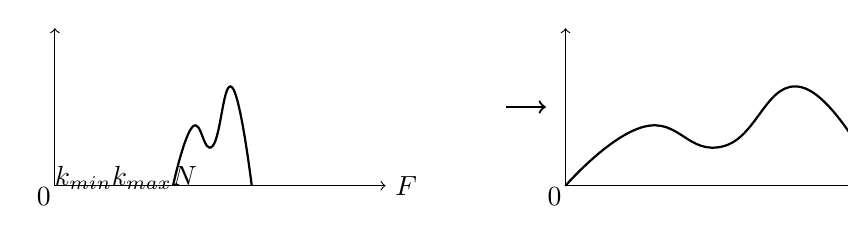
\begin{tikzpicture}
               \draw[->] (0,0) node[yshift=-4, xshift = -4] {0} -- (4.2,0) node[right] {$F$};
               \draw[->] (0,0) -- (0,2);
               \draw[thick] plot [smooth, tension = 0.8] coordinates {(1.5,0) (1.75,0.75) (2,0.5) (2.25,1.25) (2.5,0)};
               \tvmark{1.5}{0}{$k_{min}$}
               \tvmark{2.5}{0}{$k_{max}$}
               \draw[->,thick] (4.25,1) -- (4.75,1);
               \draw[->] (5,0) node[yshift=-4, xshift = -4] {0} -- (9.2,0) node[right] {$F$};
               \draw[->] (5,0) -- (5,2);
               \draw[thick,shift={(5,0)}] plot [smooth, tension = 0.8] coordinates {(0,0) (1,0.75) (2,0.5) (3,1.25) (4,0)};
               \tvmark{9}{0}{$N$}
            \end{tikzpicture}
        \end{center}

        \begin{center}
            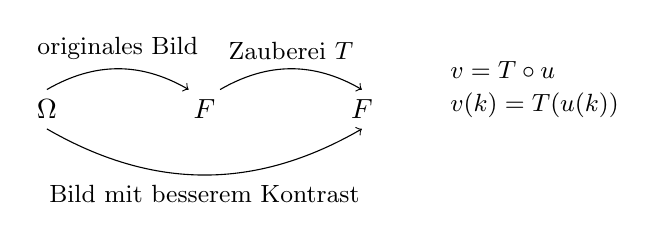
\begin{tikzpicture}
                \draw[->] (0,0) node[below] {$\Omega$} to[bend left] node[above] {\small originales Bild} (1.8,0);
                \draw (2,0) node[below] {$F$};
                \draw[->] (2.2,0) to[bend left] node[above] {\small Zauberei $T$} (4,0) node[below] {$F$};
                \draw[->] (0,-0.5) to[bend right] node[below] {\small Bild mit besserem Kontrast} (4,-0.5);
                \draw[text width = 2.3cm] (5,0) node[right] {\small $v = T \circ u$\\ $v(k)=T(u(k)) $};
            \end{tikzpicture}
        \end{center}

        \pa{1. Idee: Kontrastdehnung}\\
        $T$ \quo{lineare} Abbildung, so dass $T(k_{min})=0$ und $T(k_{max})=N$:
        \[T(k) = \frac{k - k_{min}}{k_{max} - k_{min}} N \text{, kontinuierlicher Farbraum}\]
        \[T(k) = \left[\frac{k - k_{min}}{k_{max} - k_{min}} N \right] \text{, diskreter Farbraum}\]

        \underline{Beispiel:} $k_{\min} = 20$ und $k_{\max}=102$

        \begin{center}
            \begin{tikzpicture}
                \draw[->] (0,0) node[yshift=-4, xshift = -4] {0} -- (6,0) node[right] {$F$};
                \draw[->] (0,0) -- (0,3);
                \tlbar{0.75}{0}{1}{20}{4}
                \tlbar{1.5}{0}{1.25}{40}{6}
                \tvnmark{2.25}{0}{...}
                \tlbar{3}{0}{1.75}{99}{10}
                \tlbar{3.4}{-0.3}{2.75}{100}{20}
                \tlbar{3.8}{0}{2.25}{101}{15}
                \tlbar{4.2}{-0.3}{1.125}{102}{5}
                \tvnmark{4.8}{0}{...}
                \tvmark{5.5}{0}{255}
                \draw[->, thick, text width = 2cm] (6.5,1.5) -- node[above] {\footnotesize Lineare Transformation $T$} (7.5,1.5);
                \draw[->] (8,0) node[yshift=-4, xshift = -4] {0} -- (13,0) node[right] {$F$};
                \draw[->] (8,0) -- (8,3);
                \tlbar{8}{0}{1}{}{4}% \tlbar{8.25}{0}{1}{3}{4}
                \tvnmark{8.75}{0}{...}
                \tlbar{9.25}{0}{1.75}{64}{6}
                \tvnmark{9.75}{0}{...}
                \tlbar{10.75}{0}{1.75}{246}{10}
                \tlbar{11.25}{-0.3}{2.75}{249}{20}
                \tlbar{11.75}{0}{2.25}{252}{15}
                \tlbar{12.4}{0}{1.125}{}{5}
                \tvmark{12.4}{0}{255}
                \draw[] (1.5,2.25) node[] {$\abs{\Omega}=60$};
                \draw (10.5,-0.8) ;%node[below] {\footnotesize $k_{min} =19, \ k_{max}=103$};
            \end{tikzpicture}
        \end{center}

        Dieses brint jedoch wenig, falls das Histogramm bereits voll ausgedehnt ist.

        \pa{2. Idee: Nicht-lineare Kontrastdehnung}\\
            Dieses mal setzen wir $\displaystyle T(k) =\left[ \frac{N}{\abs{\Omega}} \sum_{l=0}^{k}H_u(l) \right]$ für einen diskreten Farbraum und erhalten:

            \begin{center}
                \begin{tikzpicture}
                    \draw[->] (0,0) node[yshift=-4, xshift = -4] {0} -- (8,0) node[right] {$F$};
                    \draw[->] (0,0) -- (0,3);
                    \draw[decorate,decoration={brace,amplitude=2pt,mirror}] (0,-0.2) -- node[below] {\small $\frac{4}{60} N$} (1,-0.2);
                    \tlbar{1}{0}{1}{}{4}
                    \draw[decorate,decoration={brace,amplitude=2pt,mirror}] (1,-0.2) -- node[below] {\small $\frac{6}{60} N$} (2.5,-0.2);
                    \tlbar{2.5}{0}{1.25}{}{6}
                    \draw[decorate,decoration={brace,amplitude=2pt,mirror}] (2.5,-0.2) -- node[below] {\small $\frac{10}{60} N$} (4.5,-0.2);
                    \tlbar{4.5}{0}{1.75}{}{10}
                    \draw[decorate,decoration={brace,amplitude=2pt,mirror}] (4.5,-0.2) -- node[below] {\small $\frac{20}{60} N$} (7,-0.2);
                    \tlbar{7}{0}{2.5}{}{20}
                    \tvnmark{7.5}{0}{...}
                \end{tikzpicture}
            \end{center}
        $T$ lässt sich auch alternativ ausdrücken durch
        \[ T(k)=\left[ \mathcal H_u(\{0,...,k\}) \right]. \]
        Und somit folgt, dass für den kontinuierlichen Fall $T$ durch
        \[ T(k) = \frac{N}{\abs{\Omega}} \mathcal H_u((0,k))\]
        definiert werden kann. 
        Allgemein heißt der Prozess \textbf{Histogramm - equalization}\index{Histogramm - equalization}.
    \subsection{Anwendung: SW-Konvertierung}
        Aufgabe: Graustufenbild $\to$ SW-Bild.\\
        Nützlich etwa bei Objekterkennung/Segmentierung.

        Idee: Das Histogramm an einem gewissen \textbf{Schwellenwert}\index{Schwellenwert} $t$ spalten:

        \begin{center}
            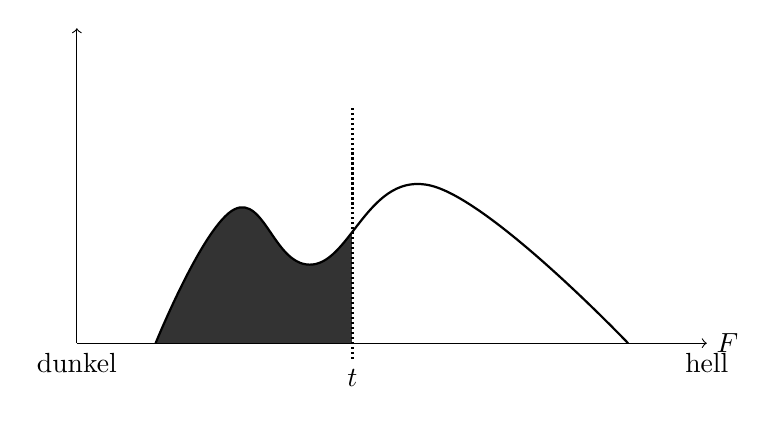
\begin{tikzpicture}
                \fill[black!80](0.1,0) rectangle (3.5,3);
                \fill [white] (0.05,0) -- plot [smooth, tension = 0.7] coordinates {(1,0) (2,1.7) (3,1) (4.5,2) (7,0)} -- (7.5,3.5) -- (0.1,3.5)  -- cycle;
                \draw[->] (0,0) node[below] {dunkel} -- (8,0) node[below] {hell} node[right] {$F$};
                \draw[->] (0,0) -- (0,4);
                \draw[thick] plot [smooth, tension = 0.7] coordinates {(1,0) (2,1.7) (3,1) (4.5,2) (7,0)};
                \draw[densely dotted,thick] (3.5,-0.2) node[below] {$t$} -- (3.5,3);
            \end{tikzpicture}
        \end{center}
        Also setze nun für $t \in F$:
    \begin{align*}
    \text{schwarz} &= \left\{k \in F \mid k \leq t \right\} \\
    \text{weiß} &= \left\{k \in F \mid k >t \right\}
    \end{align*}
     Graustufenbild $u$ $\longrightarrow$ schwarz/weiß Bild $\tilde u$:
        \[\tilde u(x) = \begin{cases}
            0, \ u(x) \in \text{schwarz}\\
            1, \ u(x) \in \text{weiß}
        \end{cases} \Rightarrow \, \tilde F = \{0,1\}.\]

        \pa{Methoden um diesen Schwellenwert $t$ zu wählen:}

        \begin{enumerate}
            \item \textbf{Shape based Methods}\index{Shape based Methods}:\\
                Falls das Histogramm von $u$ \textbf{bimodal}\index{bimodal} ist, also die Form:
            \begin{center}
                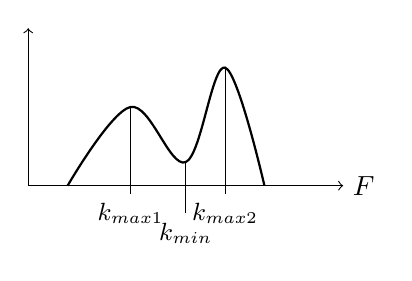
\begin{tikzpicture}
                    \draw[->] (0,0) -- (4,0) node[right] {$F$};
                    \draw[->] (0,0) -- (0,2);
                    \draw[thick] plot [smooth, tension = 0.6] coordinates {(0.5,0) (1.3,1) (2,0.3) (2.5,1.5) (3,0)};
                    \draw (1.3,-0.1) node[below] {\small $k_{max 1}$} -- (1.3,1);
                    \draw (2,-0.35) node[below] {\small $k_{min}$} -- (2,0.3);
                    \draw (2.5,-0.1) node[below] {\small $k_{max 2}$} -- (2.5,1.5);
                \end{tikzpicture}
            \end{center}
            hat, dann wähle:
            \[t \coloneqq k_{min}\]
            \[\text{oder} \ t \coloneqq  \frac{k_{max 1} + k_{max 2}}{2}\]
        \item \textbf{Otsu's Verfahren}\index{Otsu's Verfahren} (1979):\\
            Vorher einige Definitionen.\\
            Die \textbf{Masse}\index{Masse}:
            \[m_{\text{schwarz}}  \coloneqq  \sum_{k \,\in\, \text{schwarz}} H_u(k)\]
            \[m_{\text{weiß}}  \coloneqq  \sum_{k \,\in\, \text{weiß}} H_u(k)\]
            Der \textbf{Mittelwert}\index{Mittelwert}:
            \[\mu_{\text{schwarz}}  \coloneqq  \frac{\displaystyle \sum_{k \in \text{schwarz}} k \C H_u(k) }{\displaystyle \sum_{k \in \text{schwarz}}H_u(k)} = \frac{\displaystyle \sum_{k \in \text{schwarz}} k \C H_u(k) }{m_{\text{schwarz}}}\]
            \[\mu_{\text{weiß}}  \coloneqq  \frac{\displaystyle \sum_{k \in \text{weiß}} k \C H_u(k) }{\displaystyle \sum_{k \in \text{weiß}}H_u(k)} = \frac{\displaystyle \sum_{k \in \text{weiß}} k \C H_u(k) }{m_{\text{weiß}}}\]
            Die \textbf{Varianz}\index{Varianz}:
            \[\sigma^2_{\text{schwarz}} = \sum_{k \in \text{schwarz}} (k - \mu_{\text{schwarz}})^2 \C H_u(k)\]
            \[\sigma^2_{\text{weiß}} = \sum_{k \in \text{weiß}} (k - \mu_{\text{weiß}})^2 \C H_u(k)\]
            Nun lautet Otsu's Methode: $\sigma^2_{\text{schwarz}} + \sigma^2_{\text{weiß}} \overset{t}{\rightarrow} \text{min}$.
        \item \textbf{Median}\index{Median}:\\
            Wähle $t$ so, dass $m_{\text{schwarz}} = m_{\text{weiß}}$.
        \item \textbf{Isodata Algorithmus}\index{Isodata Algorithmus} (1970s):\\
            Wähle t so, dass $\displaystyle t = \frac{\mu_{\text{schwarz}} + \mu_{\text{weiß}}}{2} =: f(t)$.\\
            Diese Gleichung ist bereits eine \textbf{Fixpunktgleichung}\index{Fixpunktgleichung} und eine Lösung kann, etwa mit einer \mim{Fixpunktiteration} approximiert werden, das heißt $t_{n+1}  \coloneqq  f(t_n)$.
            \begin{center}
                \begin{tikzpicture}%TODO fixpunkt iteration in Grafik?
                    \draw[->] (0,0) node[below] {0} -- (0,5) node[above] {y};
                    \draw[->] (0,0) -- (5,0)node[right] {x};
                    \draw (-0.1,4.5) node[left] {N} -- (4.5,4.5);
                    \draw (4.5,-0.1) node[below] {N} -- (4.5,4.5);
                    \draw[name path = P1] (-0.1,-0.1) -- node[below,sloped, pos = 0.7] {$y=x$} (4.6,4.6);
                    \coordinate (A) at (0.5,0.5);
                    \draw[thick, name path = P2] plot [smooth, tension = 0.8] coordinates {(0,0.5) (0.5,0.7) (1,1.1) (2, 1.7) (2.8, 3.1) (4.5,4.25)};
                    \draw (3,3.7) node[rotate = 35] {$y = f(x)$};
                    \fill[name intersections={of=P1 and P2}]
                    (intersection-1) circle (1.5pt) node {}
                    (intersection-2) circle (1.5pt) node {}
                    (intersection-3) circle (1.5pt) node {};
                \end{tikzpicture}
            \end{center}
        \end{enumerate}

        \pa{Matlab Beispiel}:\\
        \begin{lstlisting}
u=imread('liftingbody.png');
t=greythresh(u);%uses Otsu's method
v=im2bn(u,t);
imshow(v);
        \end{lstlisting}

        Einige dieser Verfahren können auch erweitert werden, so dass ein Graustufenbild nicht nur in zwei, sondern in $M$ Farben zerlegt werden kann. Im allgemeinen werden dann $M-1$ thresholds benötigt.

        \begin{enumerate}
            \item \pa{Shape based}:\\
            \begin{center}
                \begin{tikzpicture}
                    \draw (0,0) -- (0,2);
                    \draw (0,0) -- (6,0);
                    \draw[thick, name path = P2] plot [smooth, tension = 0.7] coordinates {(0.5,0) (1,1) (1.5,0.2) (2, 0.9) (2.5, 0.5) (3.25,1.5) (4,0.5) (4.5,1.2) (5,0)};
                    \draw (1,-0.1) node[below] {$t_1$} -- (1,1);
                    \draw (2,-0.1) node[below] {$t_2$} -- (2,0.9);
                    \draw (3.25,-0.1) node[below] {$t_3$} -- (3.25,1.5);
                    \draw (4.5,-0.1) node[below] {$t_4$} -- (4.5,1.2);
                \end{tikzpicture}
            \end{center}
            \ \\
            \item \pa{Otsu's Verfahren}:\\
            Farbklassen:
            \[ F_1 = \{ k : k \leq t_1\}\]
            \[ F_2 = \{ k : t_1 < k \leq t_2\}\]
            \[\vdots\]
            \[ F_M = \{ k : t_{M-1} < k \}\]
            Und wie zuvor: $\sigma_1^2 + ... + \sigma_M^2 \to $ min
            \item \pa{Median}:\\
            Zerteile $F$ in M Quantile gleicher Masse.
            \item \pa{Isodata}:\\
            Hierzu existiert keine bekannte Verallgemeinerung auf $M$ Farbklassen.
        \end{enumerate}

        \pa{Matlab code}:\\
        \begin{lstlisting}
u=imread('Circles Bright Dark.png');
t=multithresh(u,M-1);
v=imquantize(u,t);
w=label2rgb(u,t);
imshow(w);
        \end{lstlisting}
